\documentclass[]{article}
\usepackage{lmodern}
\usepackage{amssymb,amsmath}
\usepackage{ifxetex,ifluatex}
\usepackage{fixltx2e} % provides \textsubscript
\ifnum 0\ifxetex 1\fi\ifluatex 1\fi=0 % if pdftex
  \usepackage[T1]{fontenc}
  \usepackage[utf8]{inputenc}
\else % if luatex or xelatex
  \ifxetex
    \usepackage{mathspec}
  \else
    \usepackage{fontspec}
  \fi
  \defaultfontfeatures{Ligatures=TeX,Scale=MatchLowercase}
\fi
% use upquote if available, for straight quotes in verbatim environments
\IfFileExists{upquote.sty}{\usepackage{upquote}}{}
% use microtype if available
\IfFileExists{microtype.sty}{%
\usepackage{microtype}
\UseMicrotypeSet[protrusion]{basicmath} % disable protrusion for tt fonts
}{}
\usepackage[margin=1in]{geometry}
\usepackage{hyperref}
\hypersetup{unicode=true,
            pdftitle={Re: Mining human prostate cancer datasets: The "camcAPP" shiny app},
            pdfauthor={Mark J. Dunning\^{}1, Sarah L. Vowler\^{}1, Emilie Lalonde\^{}\{2,3\}, Helen Ross-Adams\^{}4, Paul C. Boutros\^{}\{2,3\}, Ian G. Mills\^{}5, Andy G. Lynch\^{}1 and Alastair D. Lamb\^{}\{1,6\}, on behalf of the CamCaP Study Group},
            pdfborder={0 0 0},
            breaklinks=true}
\urlstyle{same}  % don't use monospace font for urls
\usepackage{color}
\usepackage{fancyvrb}
\newcommand{\VerbBar}{|}
\newcommand{\VERB}{\Verb[commandchars=\\\{\}]}
\DefineVerbatimEnvironment{Highlighting}{Verbatim}{commandchars=\\\{\}}
% Add ',fontsize=\small' for more characters per line
\usepackage{framed}
\definecolor{shadecolor}{RGB}{248,248,248}
\newenvironment{Shaded}{\begin{snugshade}}{\end{snugshade}}
\newcommand{\KeywordTok}[1]{\textcolor[rgb]{0.13,0.29,0.53}{\textbf{{#1}}}}
\newcommand{\DataTypeTok}[1]{\textcolor[rgb]{0.13,0.29,0.53}{{#1}}}
\newcommand{\DecValTok}[1]{\textcolor[rgb]{0.00,0.00,0.81}{{#1}}}
\newcommand{\BaseNTok}[1]{\textcolor[rgb]{0.00,0.00,0.81}{{#1}}}
\newcommand{\FloatTok}[1]{\textcolor[rgb]{0.00,0.00,0.81}{{#1}}}
\newcommand{\ConstantTok}[1]{\textcolor[rgb]{0.00,0.00,0.00}{{#1}}}
\newcommand{\CharTok}[1]{\textcolor[rgb]{0.31,0.60,0.02}{{#1}}}
\newcommand{\SpecialCharTok}[1]{\textcolor[rgb]{0.00,0.00,0.00}{{#1}}}
\newcommand{\StringTok}[1]{\textcolor[rgb]{0.31,0.60,0.02}{{#1}}}
\newcommand{\VerbatimStringTok}[1]{\textcolor[rgb]{0.31,0.60,0.02}{{#1}}}
\newcommand{\SpecialStringTok}[1]{\textcolor[rgb]{0.31,0.60,0.02}{{#1}}}
\newcommand{\ImportTok}[1]{{#1}}
\newcommand{\CommentTok}[1]{\textcolor[rgb]{0.56,0.35,0.01}{\textit{{#1}}}}
\newcommand{\DocumentationTok}[1]{\textcolor[rgb]{0.56,0.35,0.01}{\textbf{\textit{{#1}}}}}
\newcommand{\AnnotationTok}[1]{\textcolor[rgb]{0.56,0.35,0.01}{\textbf{\textit{{#1}}}}}
\newcommand{\CommentVarTok}[1]{\textcolor[rgb]{0.56,0.35,0.01}{\textbf{\textit{{#1}}}}}
\newcommand{\OtherTok}[1]{\textcolor[rgb]{0.56,0.35,0.01}{{#1}}}
\newcommand{\FunctionTok}[1]{\textcolor[rgb]{0.00,0.00,0.00}{{#1}}}
\newcommand{\VariableTok}[1]{\textcolor[rgb]{0.00,0.00,0.00}{{#1}}}
\newcommand{\ControlFlowTok}[1]{\textcolor[rgb]{0.13,0.29,0.53}{\textbf{{#1}}}}
\newcommand{\OperatorTok}[1]{\textcolor[rgb]{0.81,0.36,0.00}{\textbf{{#1}}}}
\newcommand{\BuiltInTok}[1]{{#1}}
\newcommand{\ExtensionTok}[1]{{#1}}
\newcommand{\PreprocessorTok}[1]{\textcolor[rgb]{0.56,0.35,0.01}{\textit{{#1}}}}
\newcommand{\AttributeTok}[1]{\textcolor[rgb]{0.77,0.63,0.00}{{#1}}}
\newcommand{\RegionMarkerTok}[1]{{#1}}
\newcommand{\InformationTok}[1]{\textcolor[rgb]{0.56,0.35,0.01}{\textbf{\textit{{#1}}}}}
\newcommand{\WarningTok}[1]{\textcolor[rgb]{0.56,0.35,0.01}{\textbf{\textit{{#1}}}}}
\newcommand{\AlertTok}[1]{\textcolor[rgb]{0.94,0.16,0.16}{{#1}}}
\newcommand{\ErrorTok}[1]{\textcolor[rgb]{0.64,0.00,0.00}{\textbf{{#1}}}}
\newcommand{\NormalTok}[1]{{#1}}
\usepackage{longtable,booktabs}
\usepackage{graphicx,grffile}
\makeatletter
\def\maxwidth{\ifdim\Gin@nat@width>\linewidth\linewidth\else\Gin@nat@width\fi}
\def\maxheight{\ifdim\Gin@nat@height>\textheight\textheight\else\Gin@nat@height\fi}
\makeatother
% Scale images if necessary, so that they will not overflow the page
% margins by default, and it is still possible to overwrite the defaults
% using explicit options in \includegraphics[width, height, ...]{}
\setkeys{Gin}{width=\maxwidth,height=\maxheight,keepaspectratio}
\IfFileExists{parskip.sty}{%
\usepackage{parskip}
}{% else
\setlength{\parindent}{0pt}
\setlength{\parskip}{6pt plus 2pt minus 1pt}
}
\setlength{\emergencystretch}{3em}  % prevent overfull lines
\providecommand{\tightlist}{%
  \setlength{\itemsep}{0pt}\setlength{\parskip}{0pt}}
\setcounter{secnumdepth}{0}
% Redefines (sub)paragraphs to behave more like sections
\ifx\paragraph\undefined\else
\let\oldparagraph\paragraph
\renewcommand{\paragraph}[1]{\oldparagraph{#1}\mbox{}}
\fi
\ifx\subparagraph\undefined\else
\let\oldsubparagraph\subparagraph
\renewcommand{\subparagraph}[1]{\oldsubparagraph{#1}\mbox{}}
\fi

%%% Use protect on footnotes to avoid problems with footnotes in titles
\let\rmarkdownfootnote\footnote%
\def\footnote{\protect\rmarkdownfootnote}

%%% Change title format to be more compact
\usepackage{titling}

% Create subtitle command for use in maketitle
\newcommand{\subtitle}[1]{
  \posttitle{
    \begin{center}\large#1\end{center}
    }
}

\setlength{\droptitle}{-2em}
  \title{Re: Mining human prostate cancer datasets: The \("\)camcAPP\("\) shiny
app}
  \pretitle{\vspace{\droptitle}\centering\huge}
  \posttitle{\par}
  \author{Mark J. Dunning\(^1\), Sarah L. Vowler\(^1\), Emilie Lalonde\(^{2,3}\),
Helen Ross-Adams\(^4\), Paul C. Boutros\(^{2,3}\), Ian G. Mills\(^5\),
Andy G. Lynch\(^1\) and Alastair D. Lamb\(^{1,6}\), on behalf of the
CamCaP Study Group}
  \preauthor{\centering\large\emph}
  \postauthor{\par}
  \date{}
  \predate{}\postdate{}

\usepackage[labelfont=bf]{caption}

\begin{document}
SUPPLEMENTARY MATERIALS

Application Manual


{\let\newpage\relax\maketitle}

\section{Introduction}\label{introduction}

The camcAPP is implemented in R as a Shiny application (Chang et al.
2017). Shiny allows for the development of data applications with no
need for web-development skills. camcAPP enables the creation of
publication-ready figures and tables for a number of prostate cancer
data sets through an intuitive online interface to the underlying R
code.

\section{Details of specific panels and
functionality}\label{details-of-specific-panels-and-functionality}

\subsection{Data Input Panel}\label{data-input-panel}

There are two tasks to complete in the Data Input panel: Specification
of a set of genes to study, and specification of the data set in which
to study them (expression analyses only). The data set is specified via
the \textbf{\emph{Choose a Dataset}} drop down menu in the obvious
manner.

\begin{figure}[htbp]
\centering
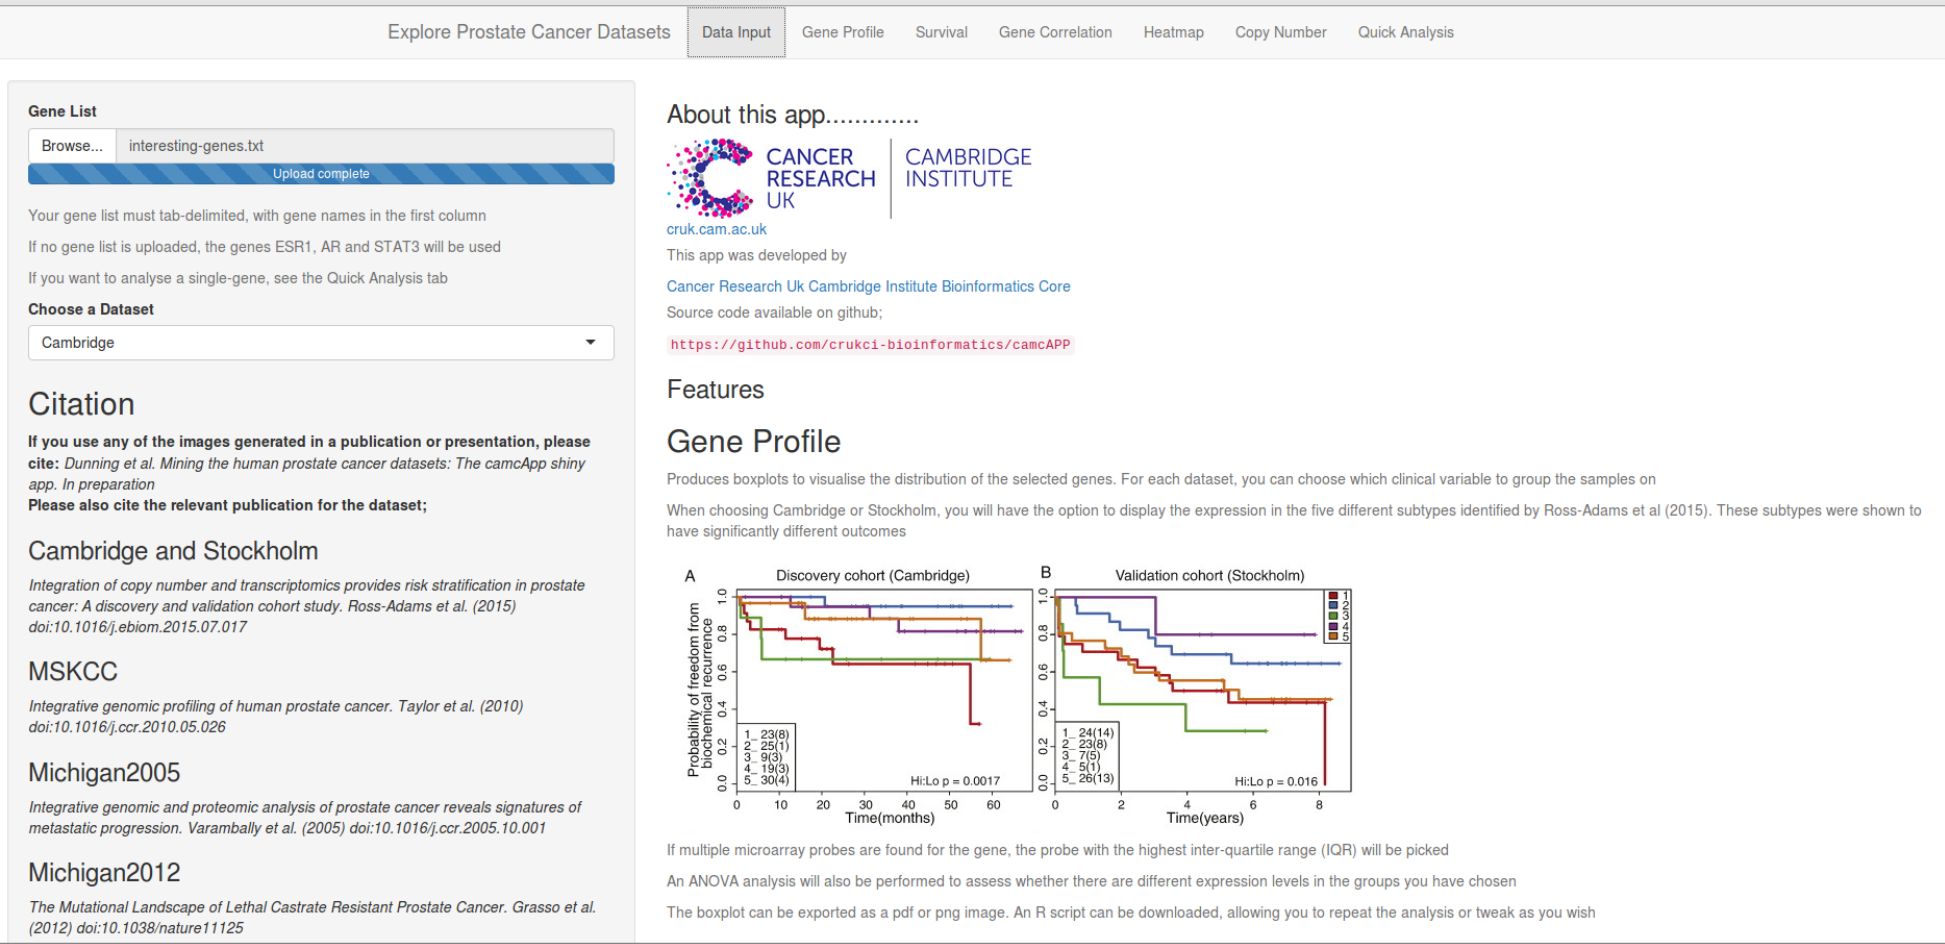
\includegraphics{Figure1.png}
\caption{Entry point to camcAPP, including the upload point for gene
lists, selecting a cohort and citation information}
\end{figure}

\subsubsection{Uploading a gene list for
interrogation}\label{uploading-a-gene-list-for-interrogation}

The gene-list must be presented in a tab-delimited file assumed to have
a column header. Only one column is required in the file, and this must
contain the offical RefSeq gene symbols that are to be used in analysis.
Each gene symbol must appear on a different row. If no list is uploaded,
a sample list of illustrative cancer-related genes is used; AR, ESR1,
HES6, MELK and STAT3. See \textbf{Figure 1}.

\subsection{Gene Profile}\label{gene-profile}

In this panel one can produce boxplots of the expression levels of the
chosen gene list across a particular study. A clinical covariate is used
to split the samples into different groups (choice of covariates will
depend on dataset). The default settings will show the Cambridge
gene-expression stratified by the subgroups identified in the CamCap
Study Group paper (Ross-Adams et al. 2015) (\textbf{Figure 2}).

\begin{figure}[htbp]
\centering
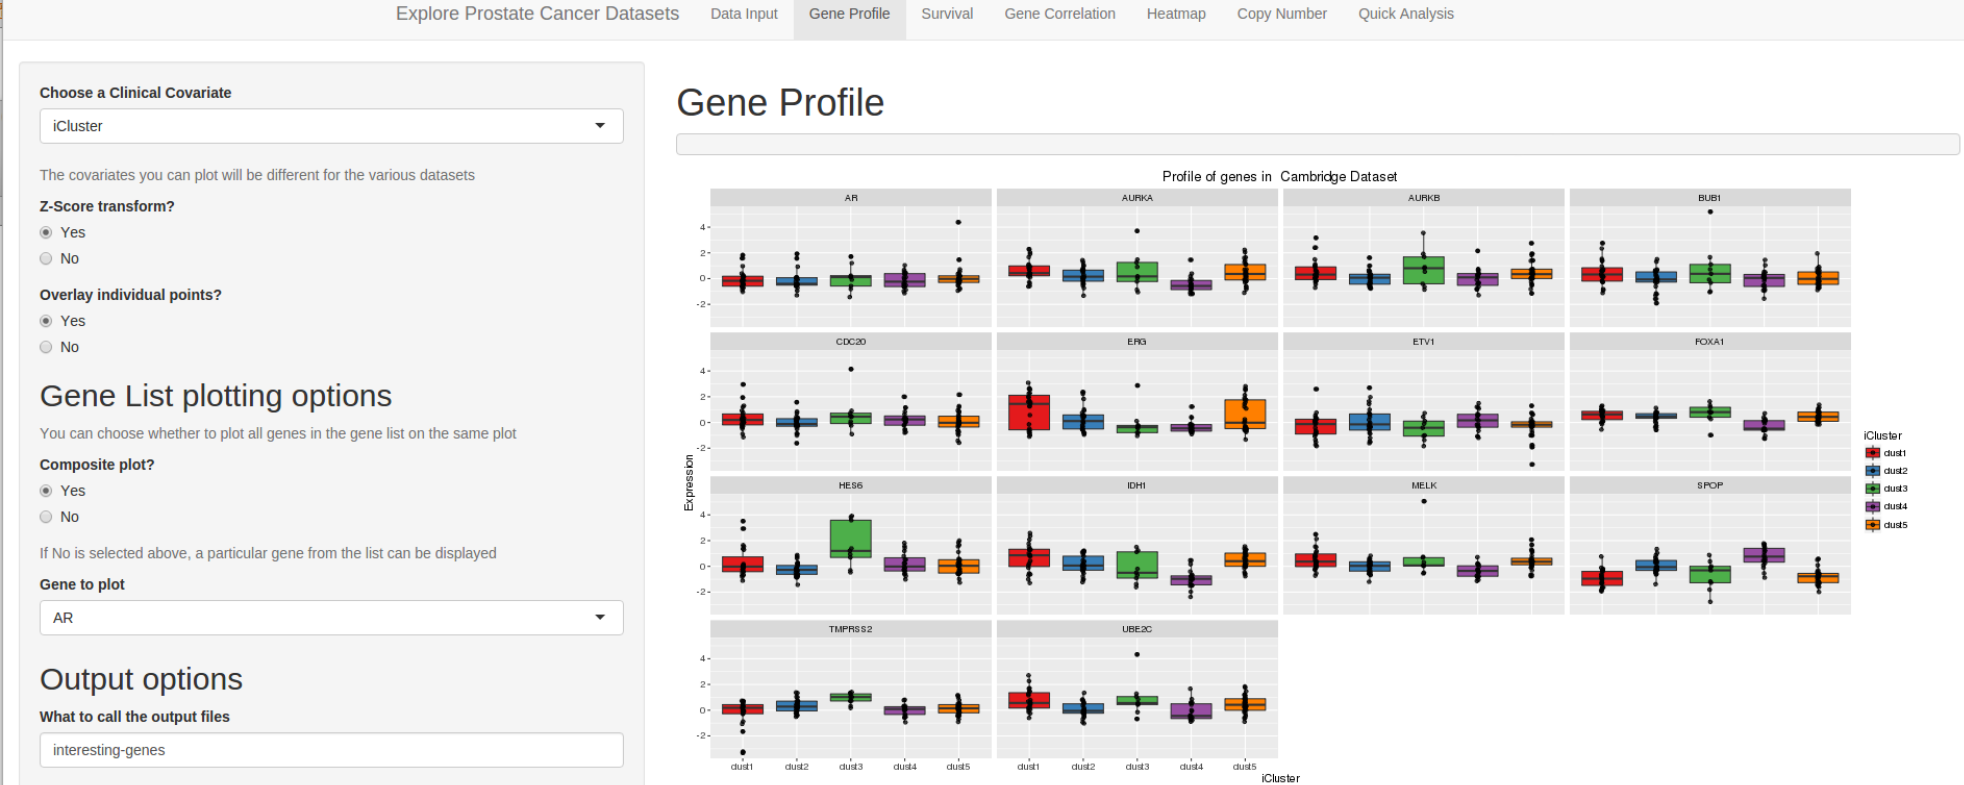
\includegraphics{Figure2.png}
\caption{Boxplots for gene expression can be created for a list of
genes. This example shows the expression profile of selected genes in
the five subgroups identified in the analysis of the CamCap Study Group
paper (Ross-Adams et al. 2015).}
\end{figure}

One can choose to tile images for all genes at once in a grid-like
display. By clicking \textbf{\emph{Composite plot?}} to
\textbf{\emph{No}} you can view a particular gene, where the gene to be
plotted is given in the \textbf{\emph{Gene to Plot}} dropdown box.

The z-score transformation will scale all genes to an average expression
level of \(0\) and standard deviation of \(1\); thus making it easier to
compare the trends of different genes.

An analysis of variance is also performed for each gene to see if there
is evidence for a change in expression level across the different
categories for selected covariate.

\subsection{Survival}\label{survival}

The \texttt{party} R package (Hothorn et al. 2006) is first used on a
gene-by-gene basis to see if the samples can be partitioned into
(typically, two) groups with distinct (p-value of \(<0.05\)) survival
profiles based on the expression levels. If no signficant partitioning
is identified, samples are assigned to low or high expression level
groups based on the median expression level of the gene.

\begin{figure}[htbp]
\centering
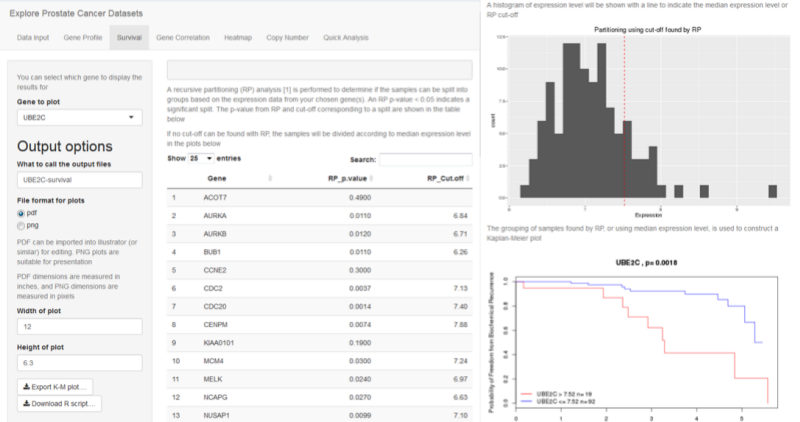
\includegraphics{Figure3.png}
\caption{Kaplan-Meier biochemical relapse-free survival plots can be
created for any selected gene from the input list in an selected
dataset.}
\end{figure}

The histogram (\textbf{Figure 3. Top Right}) shows the distribution of
expression levels for a chosen gene (defined by the \textbf{\emph{Gene
to plot}} drop-down) and vertical line to show the cut-off to be used to
assign samples to groups (either median expression level, or the cut-off
identified by recursive partitioning)

A Kaplan-Meier curve is then generated from the biochemical relapse-free
times of samples in the different groups (\textbf{Figure 3. Bottom
Right}).

Note only the Cambridge 2015, Stockholm and MSKCC dataset include the
appropriate clinical metadata to perform a survival analysis.

\subsection{Gene Correlation}\label{gene-correlation}

This panel can display scatter plots for all pairwise combinations of
genes in the selected list. Points in the scatter plots can be coloured
according to the different clinical covariates in the selected study.

\begin{figure}[htbp]
\centering
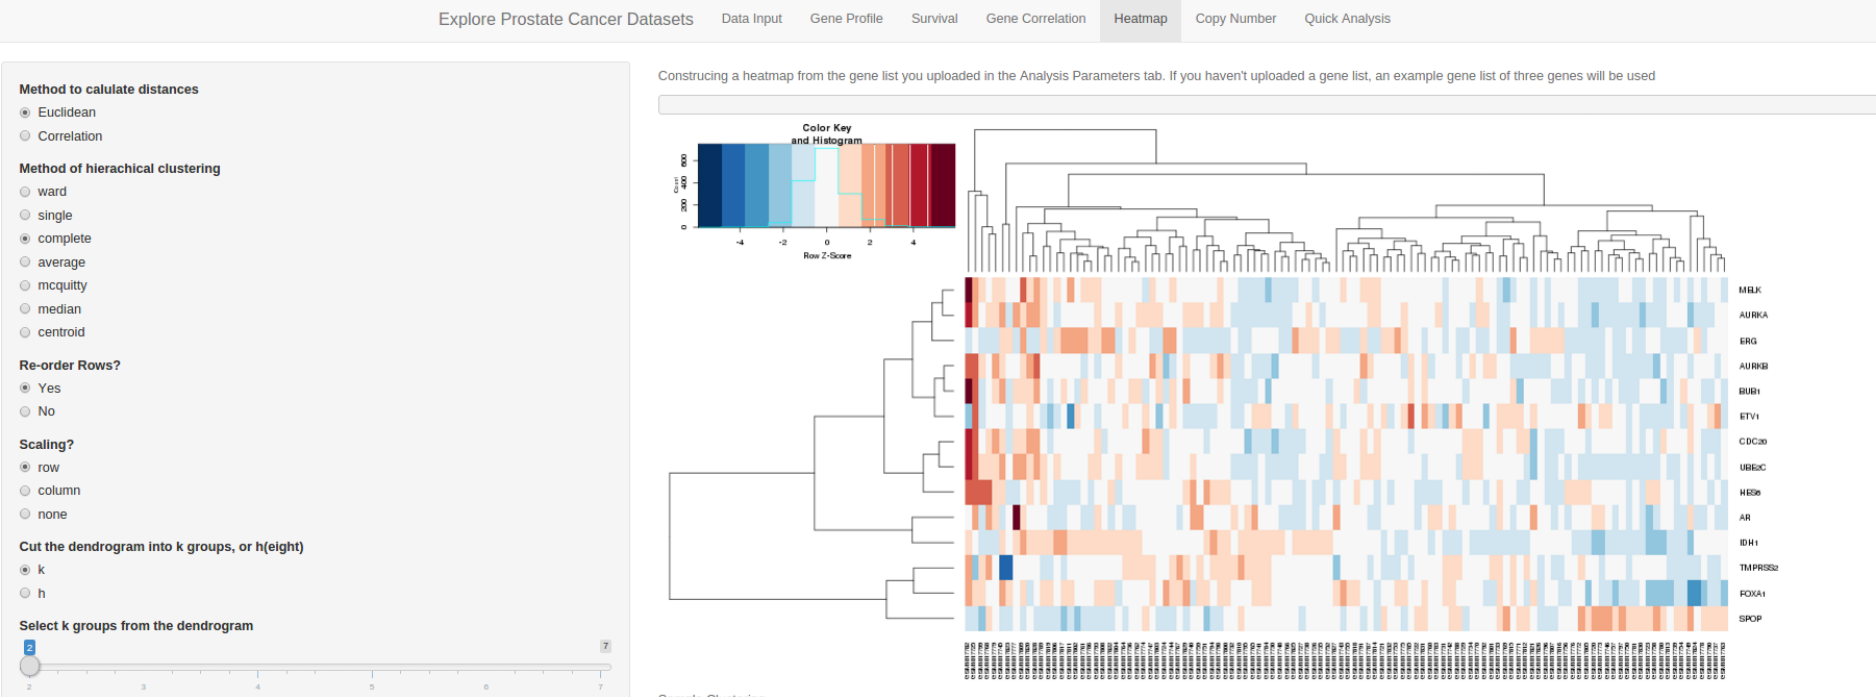
\includegraphics{Figure4.png}
\caption{Pairwise scatter plots showing the relationship between the
selected gene (STAT3) and all other members of the gene list}
\end{figure}

Alternatively, a single gene can be selected from the gene list and the
panel will be display a series of scatter plots with the expression
level of the selected gene on the y-axis, and each other gene in the
x-axis. These scatter plots will also show the value of \(r^2\) using
either Pearson or Spearman correlation (\textbf{Figure 4}).

\subsection{Heatmap}\label{heatmap}

The entire gene-list is used to cluster the samples in the chosen study,
and the resulting ordering of samples is displayed using a heatmap
(\textbf{Figure 5}). Cells in the heatmaps are coloured blue for
under-expressed genes and red for over-expressed. The default option
generate a heatmap by computing Euclidean distances and applying
hierachical clustering with complete linkage. However, other popular
methods (e.g.~correlation-based distance) are supported. Furthermore,
the rows of the heatmap (i.e.~the genes in the gene-list) can be ordered
according to the results of the clustering, or left in the order in
which they occur in the gene-list (option \textbf{\emph{Re-order
Rows?}}).

\begin{figure}[htbp]
\centering
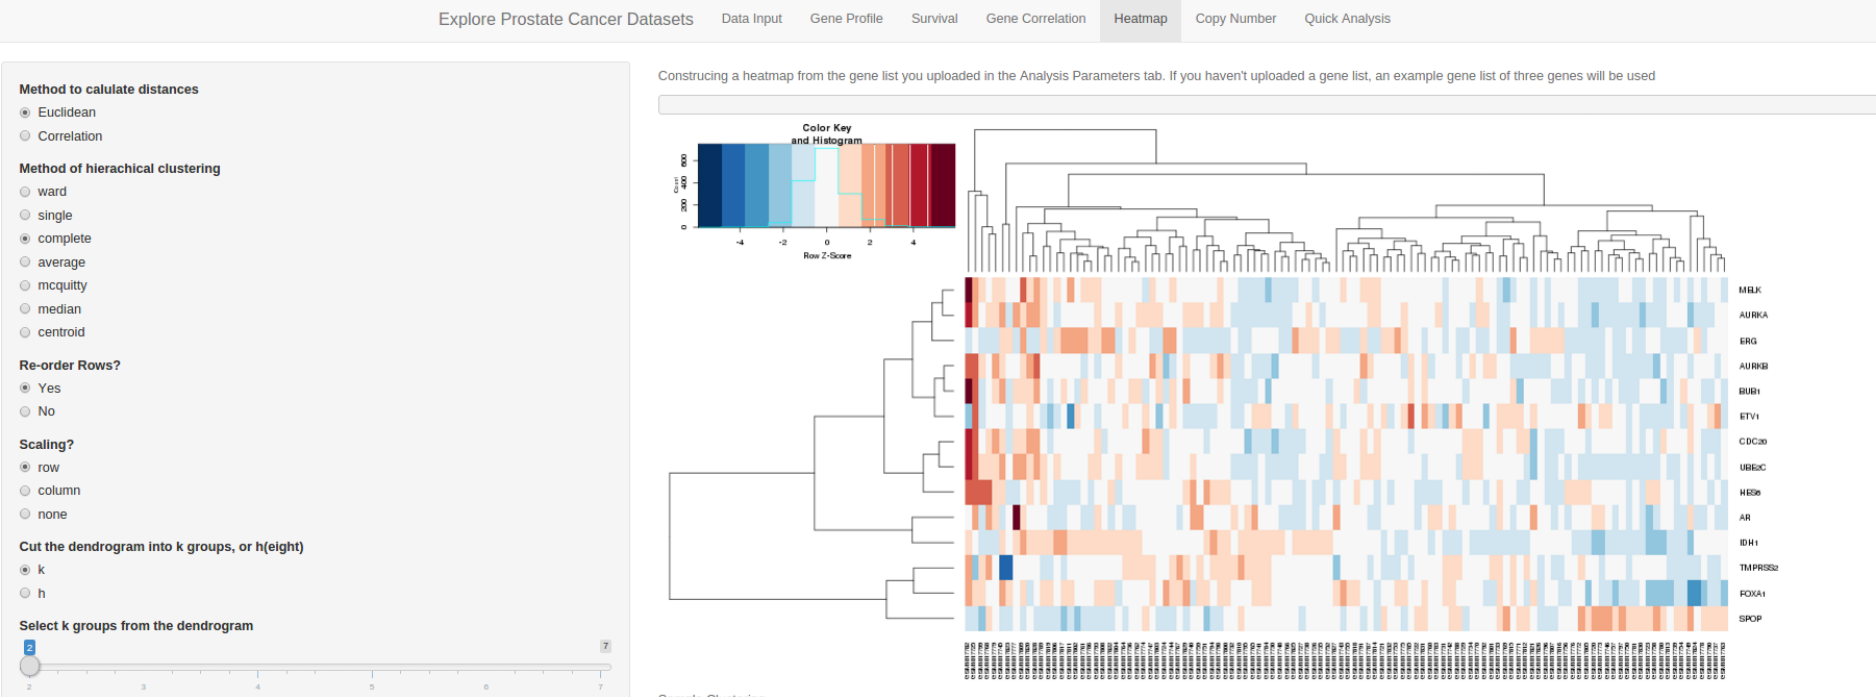
\includegraphics{Figure5.png}
\caption{Heatmaps for gene expression can be created from any of the
datasets.}
\end{figure}

We also include some basic exploratory analysis of the sample
clustering. The dendrogram of the samples can be ``cut'' at a specified
height, \(h\), (on the y-axis), or an unknown height that will yield a
pre-determined number of clusters, \(k\). The clinical characteristics
of the samples that fall into each cluster are then tabulated. Note that
the values of \(h\) and \(k\) are restricted to give between 2 and 10
clusters.

\subsection{Copy Number}\label{copy-number}

This panel allows the visualisation of copy-number calls from Cambridge,
Stockholm and MSKCC datasets. The processing of these datasets has been
previously described (Lalonde et al. 2014). The type of visualisation is
controlled by the \textbf{\emph{Type of plot to show}} drop-down menu.
Firstly, the \textbf{\emph{Frequency}} option allows one to see, on a
per-gene basis, the percentage of samples in each of the cohorts that
have an amplification or deletion of the given gene. Alternatively, the
\textbf{\emph{Frequency by Dataset}} option splits the number of samples
into different clinical subgroups and tabulates the number of per-gene
deletions and amplifcations for each subgroup.

\begin{figure}[htbp]
\centering
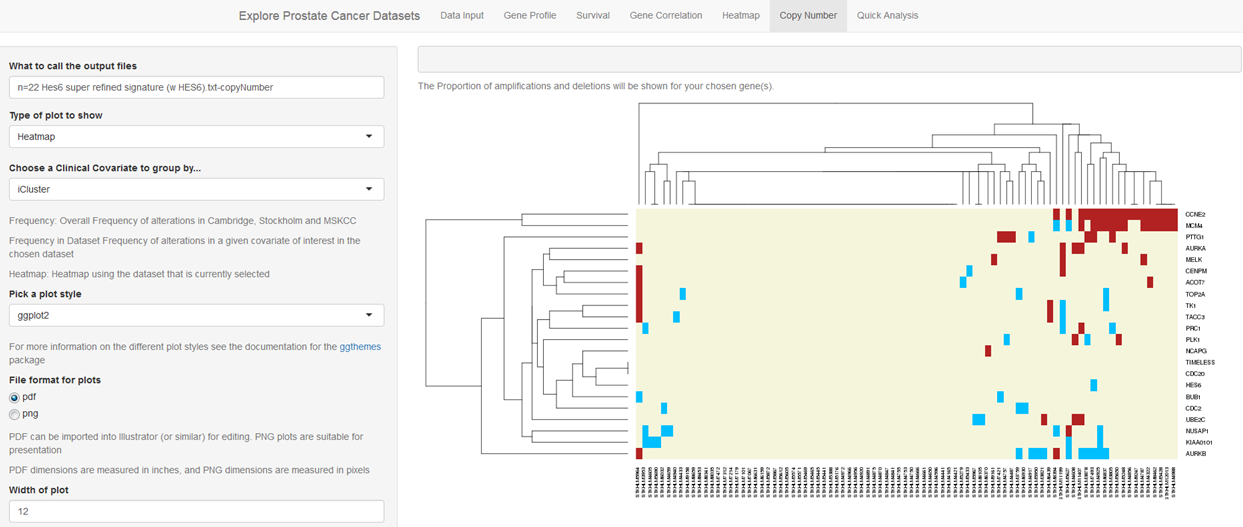
\includegraphics{Figure6.png}
\caption{Copy Number (CN) plots depicting CN gain or loss can also be
created.}
\end{figure}

Finally, the \textbf{\emph{Heatmap}} option generates a heatmap from the
copy-number calls of all selected genes in the selected cohort. This
therefore allows the user to assess whether certain genes are amplified
or deleted in the same samples (\textbf{Figure 6}).

\subsection{Quick Analysis}\label{quick-analysis}

This panel allows the boxplots, survival and copy-number analysis listed
above to be performed on a single-gene rather than a gene list. The gene
name must be entered into the text box, and the user can check whether
the name entered is a valid gene name before clicking
\textbf{\emph{Go!}} to proceed with the analysis.

\begin{figure}[htbp]
\centering
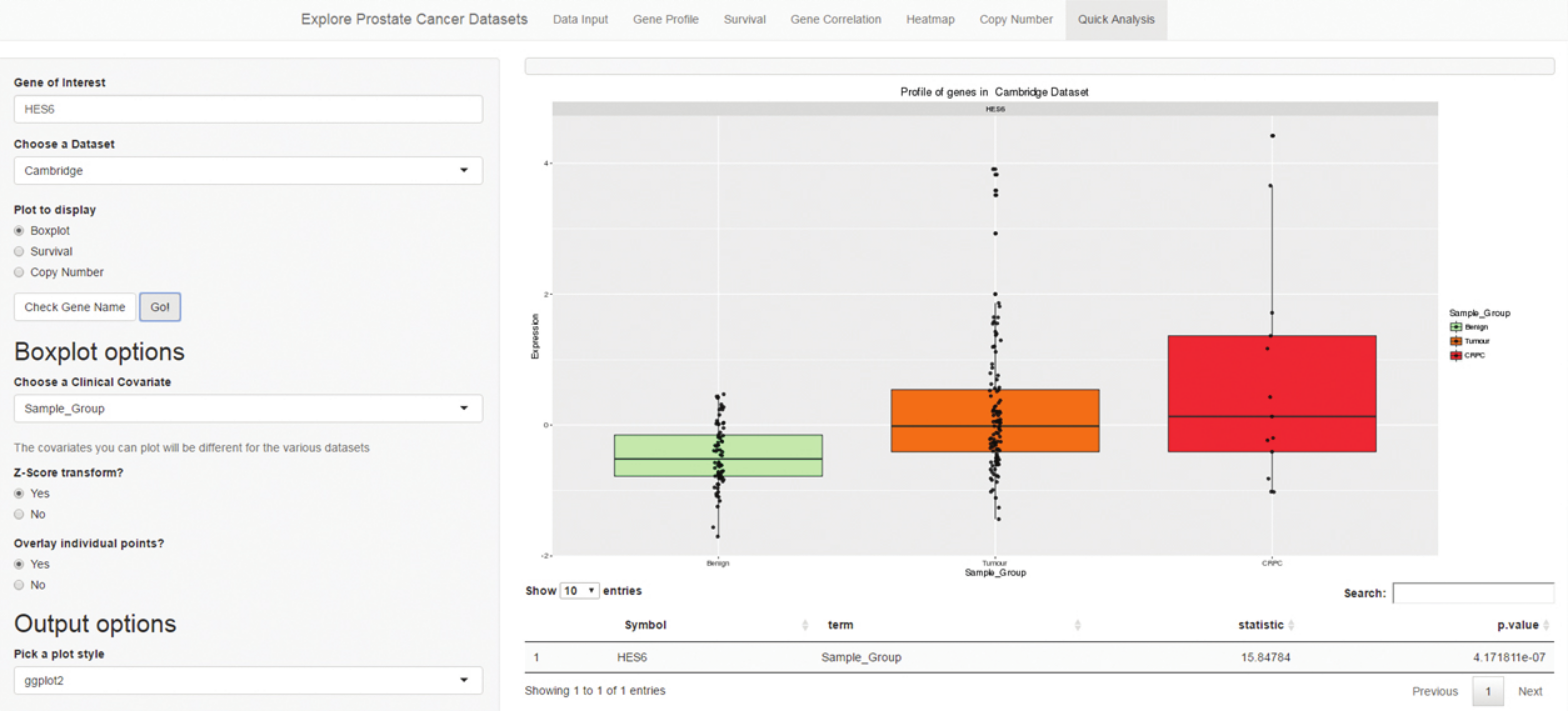
\includegraphics{Figure7.png}
\caption{The Quick Analysis tab allows for rapid spot checks for single
genes of interest focussing on relative gene expression, copy number,
and survival curves. The example shown here is a boxplot showing
relative gene expression in CRPC (castrate resistant prostate cancer),
tumour and benign tissue for HES6, a known driver of castration in
resistance (Ramos-Montoya et al. (2014))}
\end{figure}

\newpage

\section{Implementation}\label{implementation}

The source code for camcAPP is available through github (M. Dunning
2017). The \texttt{dplyr} (Wickham and Francois 2016) package is used
throughout for efficient data manipulation and graphics are generated
using \texttt{ggplot2} (Wickham 2009). Plots can be exported as PDF or
PNG file with configurable height, width and file name. Some
configuration of the background colour and grid style is also possible
with the \textbf{\emph{Pick a plot style}} drop-down box, which changes
the overall appearance of the plot using pre-defined themes in
\texttt{ggplot2} and the \texttt{ggthemes} package (Arnold 2016).

\section{Data Availability}\label{data-availability}

Each dataset that can be interrogated using camcAPP has previously been
made available through Gene Expression Omnibus (GEO). Using the GEOquery
(S. Davis and Meltzer 2007) Bioconductor package, each dataset was
downloaded and converted into a data object (\texttt{ExpressionSet})
compatible with Bioconductor (Huber et al. 2015) packages. Thus, each
dataset is also available as a Bioconductor experimental data package
and can be downloaded and interrogated independantly of camcAPP. The R
code used to download and process each dataset is available in its
respective package vignette. Below is the R code required to download
the data package for the Cambridge 2015 dataset. Datasets other than
Cambridge 2015 can be installed by replacing
\texttt{prostateCancerCamcap} with the appropriate package name. GEO
accession numbers and corresponding Bioconductor package names are given
in Table 1.

\subsection{Example of installing the prostateCancerCamcap data package
in
R}\label{example-of-installing-the-prostatecancercamcap-data-package-in-r}

\begin{Shaded}
\begin{Highlighting}[]
\KeywordTok{source}\NormalTok{(}\StringTok{"http://www.bioconductor.org/biocLite.R"}\NormalTok{)}
\KeywordTok{biocLite}\NormalTok{(}\StringTok{"prostateCancerCamcap"}\NormalTok{)}
\end{Highlighting}
\end{Shaded}

\begin{longtable}[]{@{}lll@{}}
\caption{Summary of each dataset accessible through camcAPP, its GEO
accession number and Bioconductor data package}\tabularnewline
\toprule
Dataset & GEO Accession & Bioconductor Package\tabularnewline
\midrule
\endfirsthead
\toprule
Dataset & GEO Accession & Bioconductor Package\tabularnewline
\midrule
\endhead
Cambridge 2015 & GSE70770 & prostateCancerCamcap\tabularnewline
Stockholm 2015 & GSE70769 & prostateCancerStockholm\tabularnewline
MSKCC 2010 & GSE21032 & prostateCancerTaylor\tabularnewline
Michigan 2012 & GSE35988 & prostateCancerGrasso\tabularnewline
Michigan 2005 & GSE3325 & prostateCancerVarambally\tabularnewline
\bottomrule
\end{longtable}

\subsection{Reproducible analyses using
docker}\label{reproducible-analyses-using-docker}

Docker is a system that facilitates the sharing of software in a manner
that removes dependencies on additional software (that may not be
available) and enables consistent, reproducible, research (Boettiger
2015). We provide a docker container for those that want easy access to
all the R code, packages and datasets used in the app. The latest
version of Docker is available for Windows 10 and Mac OSX 10.11 or
newer. Once Docker is install, the container to run camcAPP can be
installed and run from a terminal window as follows.

\begin{Shaded}
\begin{Highlighting}[]
\KeywordTok{docker} \NormalTok{pull markdunning/camcapp}
\KeywordTok{docker} \NormalTok{run -p 8787:8787 markdunning/camcapp}
\end{Highlighting}
\end{Shaded}

Entering the address: \texttt{http://localhost:8787} in a web-browser
will then open an RStudio session with the username and password
\texttt{rstudio}. Running the following commands in the RStudio console
will run the app.

\begin{Shaded}
\begin{Highlighting}[]
\KeywordTok{library}\NormalTok{(shiny)}
\KeywordTok{runApp}\NormalTok{(}\StringTok{"../camcAPP"}\NormalTok{)}
\end{Highlighting}
\end{Shaded}

\section*{References}\label{references}
\addcontentsline{toc}{section}{References}

\hypertarget{refs}{}
\hypertarget{ref-ggthemes}{}
Arnold, Jeffrey B. 2016. \emph{ggthemes: Extra Themes, Scales and Geoms
for 'ggplot2'}. \url{https://CRAN.R-project.org/package=ggthemes}.

\hypertarget{ref-Boettiger:2015:IDR:2723872.2723882}{}
Boettiger, Carl. 2015. ``An Introduction to Docker for Reproducible
Research.'' \emph{SIGOPS Oper. Syst. Rev.} 49 (1). New York, NY, USA:
ACM: 71--79.
doi:\href{https://doi.org/10.1145/2723872.2723882}{10.1145/2723872.2723882}.

\hypertarget{ref-shiny}{}
Chang, Winston, Joe Cheng, JJ Allaire, Yihui Xie, and Jonathan
McPherson. 2017. \emph{Shiny: Web Application Framework for R}.
\url{https://CRAN.R-project.org/package=shiny}.

\hypertarget{ref-GEOquery}{}
Davis, Sean, and Paul Meltzer. 2007. ``GEOquery: A Bridge Between the
Gene Expression Omnibus (Geo) and Bioconductor.'' \emph{Bioinformatics}
14: 1846--7.

\hypertarget{ref-github-repo}{}
Dunning, Mark. 2017. ``crukci-bioinformatics/camcAPP: Submitted
Version.''
doi:\href{https://doi.org/10.5281/zenodo.248725}{10.5281/zenodo.248725}.

\hypertarget{ref-party}{}
Hothorn, T., Hornick, K., Zeileis, and A. 2006. ``Unbiased Recursive
Partitioning.'' \emph{Journal of Computational and Graphical Statistics}
15 (3): 651--74.

\hypertarget{ref-BioC}{}
Huber, W., Carey, V. J., Gentleman, R., Anders, et al. 2015.
``Orchestrating High-Throughput Genomic Analysis with Bioconductor.''
\emph{Nature Methods} 12 (2): 115--21.
\url{http://www.nature.com/nmeth/journal/v12/n2/full/nmeth.3252.html}.

\hypertarget{ref-CopyNumber}{}
Lalonde, E., Ishkanian, A.S., Sykes, J., Fraser, et al. 2014. ``Tumour
Genomic and Microenvironmental Heterogeneity for Integrated Prediction
of 5-Year Biochemical Recurrence of Prostate Cancer: A Retrospective
Cohort Study.'' \emph{The Lancet Oncology} 15 (13): 1521--32.

\hypertarget{ref-Hes6}{}
Ramos-Montoya, A., Lamb, A.D., Russell, R., Carroll, et al. 2014. ``HES6
Drives a Critical AR Transcriptional Programme to Induce
Castration-Resistant Prostate Cancer Through Activation of an
E2F1-Mediated Cell-Cycle Network.'' \emph{EMBO Molecular Medicine} 6
(5).

\hypertarget{ref-Ross-Adams}{}
Ross-Adams, H., Lamb, A.D., Dunning, M.J., Halim, et al. 2015.
``Integration of Copy Number and Transcriptomics Provides Risk
Stratification in Prosate Cancer: A Discovery and Validation Cohort
Study.'' \emph{eBioMedicine} 2 (9): 1133--44.

\hypertarget{ref-ggplot2}{}
Wickham, Hadley. 2009. \emph{Ggplot2: Elegant Graphics for Data
Analysis}. Springer-Verlag New York. \url{http://ggplot2.org}.

\hypertarget{ref-dplyr}{}
Wickham, Hadley, and Romain Francois. 2016. \emph{Dplyr: A Grammar of
Data Manipulation}. \url{https://CRAN.R-project.org/package=dplyr}.


\end{document}
